\documentclass[11pt,a4paper]{article}
\usepackage[T1]{fontenc}
\usepackage[utf8]{inputenc}
\usepackage{lmodern}
\usepackage[margin=22mm,headheight=16pt]{geometry}
\usepackage{amsmath,amssymb,graphicx,array,longtable,booktabs}
\usepackage{microtype,xcolor,hyperref,xurl,fancyhdr}
\definecolor{Navy}{HTML}{17324D}
\definecolor{Teal}{HTML}{087F8C}
\definecolor{Gold}{HTML}{B88128}
\hypersetup{colorlinks=true,linkcolor=Navy,urlcolor=Teal,bookmarksnumbered=true,hypertexnames=false}
\setlength{\parindent}{0pt}
\setlength{\parskip}{6pt}
\setlength{\emergencystretch}{4em}
\setcounter{tocdepth}{1}
\pagestyle{fancy}\fancyhf{}
\fancyfoot[R]{\small\thepage}
\fancyfoot[L]{\small\sffamily Sharif University of Technology}
\renewcommand{\headrulewidth}{0.3pt}
\makeatletter
\renewcommand\section{\@startsection{section}{1}{\z@}{-3.2ex plus -1ex minus -.2ex}{1.6ex plus .2ex}{\normalfont\Large\sffamily\bfseries\color{Navy}}}
\renewcommand\subsection{\@startsection{subsection}{2}{\z@}{-2.5ex plus -1ex minus -.2ex}{1.2ex plus .2ex}{\normalfont\large\sffamily\bfseries\color{Teal}}}
\makeatother
\fancyhead[L]{\small\sffamily\color{Navy}Reza Sanaee Nezhad}\fancyhead[R]{\small\sffamily\color{Teal}Technical Report}\begin{document}
\begin{titlepage}\centering\vspace*{7mm}

\includegraphics[width=31mm]{assets/sharif_emblem_en.png}\par\vspace{5mm}
{\Large\sffamily\bfseries\color{Navy}SHARIF UNIVERSITY OF TECHNOLOGY\par}
\vspace{2mm}{\sffamily Department of Electrical Engineering\par}
\vspace{17mm}{\color{Teal}\rule{\linewidth}{1.4pt}}\par\vspace{6mm}
{\large\sffamily\color{Teal}TECHNICAL REPORT\par}
\vspace{8mm}{\huge\sffamily\bfseries\color{Navy}Linux Process Telemetry and Unix-Domain IPC Services\par}
\vspace{9mm}{\color{Gold}\rule{45mm}{1pt}}\par\vfill
\begin{minipage}{.88\linewidth}{\sffamily\color{Teal}AUTHOR}\par{\Large\sffamily Reza Sanaee Nezhad}\par Student ID: 401101502\par\vspace{7mm}
{\sffamily\color{Teal}INSTRUCTOR / INSTRUCTORS}\par
Dr Iman Gholampour\par\vspace{7mm}
{\sffamily\color{Teal}ACADEMIC CONTEXT}\par
Embedded Systems\par\end{minipage}\vfill
\end{titlepage}
\tableofcontents\clearpage
\section{Startup chain}

The bootloader initializes required processor, RAM, and clock resources, obtains the kernel image and hardware description from nonvolatile storage, establishes boot arguments, and transfers execution to the kernel. Platform ROM or earlier boot stages may precede this loader;\allowbreak{} it is not universally the first code executed after power-on. The kernel manages processors, memory, devices, scheduling, and networking. It initializes its own structures and drivers, mounts an initial/\allowbreak{}root filesystem, and starts the first userspace program as PID 1. The root filesystem supplies executables, configuration, libraries, and the directory structure needed by userspace. It is data and storage organization, not an executable that calls the next stage. Missing required init/\allowbreak{}root contents can prevent startup, although an initramfs may provide an earlier userspace environment. A C library such as glibc, musl, or uClibc supplies standard operations and system-call wrappers. Dynamically linked applications require a compatible runtime library and loader;\allowbreak{} static linkage changes that requirement. C+\allowbreak{}+\allowbreak{} streams additionally rely on the C+\allowbreak{}+\allowbreak{} runtime, rather than being provided by libc alone.


init/\allowbreak{}systemd configures userspace, mounts virtual filesystems, manages services, and handles PID-1 responsibilities. It can configure networking and launch daemons before the application. User applications perform the device's final function, such as control, a GUI, or data processing, and are commonly started through service definitions or init scripts.

\section{Host/target compilation and toolchains}

A normal x86/\allowbreak{}x86-64 compiler emits instructions for its configured target, which an ARM processor does not execute natively. Moving that binary to the board commonly produces an executable-format failure. Cross compilation builds a binary for the board on the development machine, for example with an appropriate ARM Linux g+\allowbreak{}+\allowbreak{} toolchain. Matching instruction-set architecture is necessary but ABI, operating-system interface, word size, runtime libraries, and floating-point ABI also matter. In this scenario the laptop is the development/\allowbreak{}build machine and the board is the execution target. Toolchain terminology can distinguish build, host, and target in more complex compiler-building situations. Native compilation uses a compatible local execution target;\allowbreak{} cross compilation selects another target configuration. The compiler translates C+\allowbreak{}+\allowbreak{} into target code. The assembler produces object files. The linker combines objects and target-compatible libraries. Kernel userspace headers define interface structures and constants;\allowbreak{} target C/\allowbreak{}C+\allowbreak{}+\allowbreak{} libraries provide the runtime. GDB with gdbserver can support remote debugging. Make tracks dependencies and avoids unnecessary recompilation, while CMake generates build descriptions and centralizes configuration. A CMake toolchain file can select cross-compilers and a target sysroot without rewriting application source.

\section{Root directories and filesystem choices}

/\allowbreak{}bin conventionally supplies essential commands such as sh, ls, and cp, although merged-/\allowbreak{}usr systems organize these through links. /\allowbreak{}etc contains system and service configuration. /\allowbreak{}lib supplies runtime libraries and, in conventional layouts, kernel modules. /\allowbreak{}dev contains device interfaces, which do not correspond one-to-one with every physical component. /\allowbreak{}var holds changing application/\allowbreak{}system state such as logs.


/\allowbreak{}proc exposes process and kernel information. /\allowbreak{}sys exposes the kernel's device/\allowbreak{}driver model and related attributes. Their content is generated through virtual filesystem interfaces;\allowbreak{} it is not an ordinary static set of files stored on flash. Reading these interfaces can change between operations, which is central to the process-monitoring exercise.


ext4 supports writable persistent data and journals metadata to assist recovery. Journaling does not guarantee that every recent application write survives power loss;\allowbreak{} synchronization and device behavior matter. Frequent writes can contribute to flash wear. SquashFS is compressed and read-only, useful for immutable system images;\allowbreak{} it avoids writes to that filesystem during ordinary operation but does not make the entire storage device immune to failures. tmpfs is temporary memory-backed storage;\allowbreak{} its data does not survive a reboot, and it can be swapped depending on system configuration. Reducing flash-backed temporary writes through tmpfs is useful only with appropriate memory/\allowbreak{}swap policy.

\section{Device Tree and overlays}

Device Tree separates board hardware description from kernel source and is especially useful for devices that cannot self-enumerate. It can describe CPU topology, memory ranges, peripheral register addresses, interrupt routing, clocks, regulators, and pin configuration. Compatible descriptions and available drivers allow one kernel build to support multiple boards, but not arbitrary hardware without matching support. An overlay modifies a base tree, for example enabling an expansion board or describing an added peripheral. The example selects i2c1, sets status to okay, and adds a BMP280 node at address 0x76 with compatible bosch,bmp280. A bootloader or supported runtime overlay mechanism can apply it without rebuilding kernel code if the corresponding driver is already available. Merely supplying an overlay cannot create a missing driver or guarantee runtime reconfiguration on every platform.

\section{Timing predictability}

Standard Linux workloads can experience scheduling delay, nonpreemptible critical sections, interrupt-disabled intervals, memory faults, reclaim/\allowbreak{}storage work, and driver/\allowbreak{}hardware interference. Kernel versions and preemption settings affect which sections can be preempted. These sources make a hard deadline guarantee a system-analysis problem rather than a label attached to a distribution. PREEMPT\_\allowbreak{}RT increases preemptibility and threads many interrupt handlers, helping reduce latency while preserving Linux libraries, drivers, and development tools. Synchronization changes and configuration can affect throughput. The experiment report characterizes it as only soft/\allowbreak{}firm real time and quotes a universal microsecond scale;\allowbreak{} those conclusions are qualified. Suitability depends on measured worst-case behavior, the platform, workload, and required bound. A split design assigns time-critical work to a microcontroller or real-time processor with an RTOS, while Linux handles networking, UI, and data. Cortex-M/\allowbreak{}Cortex-R and Cortex-A illustrate these roles. It introduces two toolchains/\allowbreak{}codebases and a communication interface, perhaps shared memory or OpenAMP. It can improve isolation, but does not confer absolute zero-jitter operation or immunity to shared power, memory, or bus faults. The recorded examples of motor control, medical functions, and high-rate signal paths motivate this split;\allowbreak{} their actual assurance depends on requirements and verified design.

\section{Unix-domain request/response implementation}

The C+\allowbreak{}+\allowbreak{} applications communicate through AF\_\allowbreak{}UNIX at /\allowbreak{}tmp/\allowbreak{}hw1\_\allowbreak{}socket. The server removes a stale pathname with unlink, creates/\allowbreak{}binds a socket, listens, and repeatedly accepts clients. It reads a command, sends the response, closes the client connection, and returns to accept. TIME uses date/\allowbreak{}time library functions;\allowbreak{} ECHO returns the text following the command. The client combines argc/\allowbreak{}argv into a request, connects, sends, reads a response, prints it, and exits. The supplied Makefile builds server and client with g+\allowbreak{}+\allowbreak{} using C+\allowbreak{}+\allowbreak{}11 and supplies a clean target. In the recorded test, TIME returned Mon Jul 6 17:\allowbreak{}33:\allowbreak{}03 2026. ECHO returned Hello Embedded Systems! in a second connection. Both terminal captures are preserved. These tests establish two successive requests in a local demonstration. They do not establish unlimited message length, complete partial-read/\allowbreak{}write handling, concurrent-client throughput, or access control. Socket-directory permissions, safe handling of stale paths, framing, maximum request size, malformed commands, and orderly cleanup are relevant extension points.

\begin{figure}[!htbp]\centering
\includegraphics[width=\linewidth,height=.72\textheight,keepaspectratio]{assets/019_p017_01.png}\caption{Diagram or recorded result: Unix-domain request/response implementation.}\label{fig:019_p017_010}\end{figure}
\begin{figure}[!htbp]\centering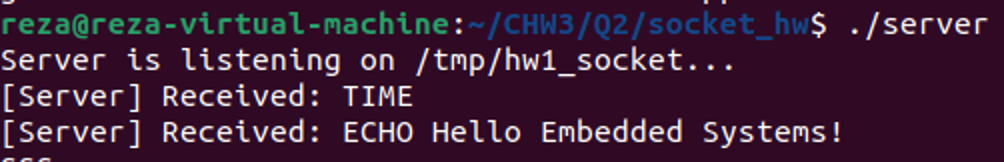
\includegraphics[width=\linewidth,height=.72\textheight,keepaspectratio]{assets/019_p018_01.png}\caption{Diagram or recorded result: Unix-domain request/response implementation.}\label{fig:019_p018_010}\end{figure}
\clearpage
\section{procwatch code organization and build}

The monitor separates main/\allowbreak{}sysinfo implementation under src and sysinfo.h under include. Both Make and CMake are supplied. Later phases add process enumeration and background-service configuration while retaining the module separation.

\begin{figure}[!htbp]\centering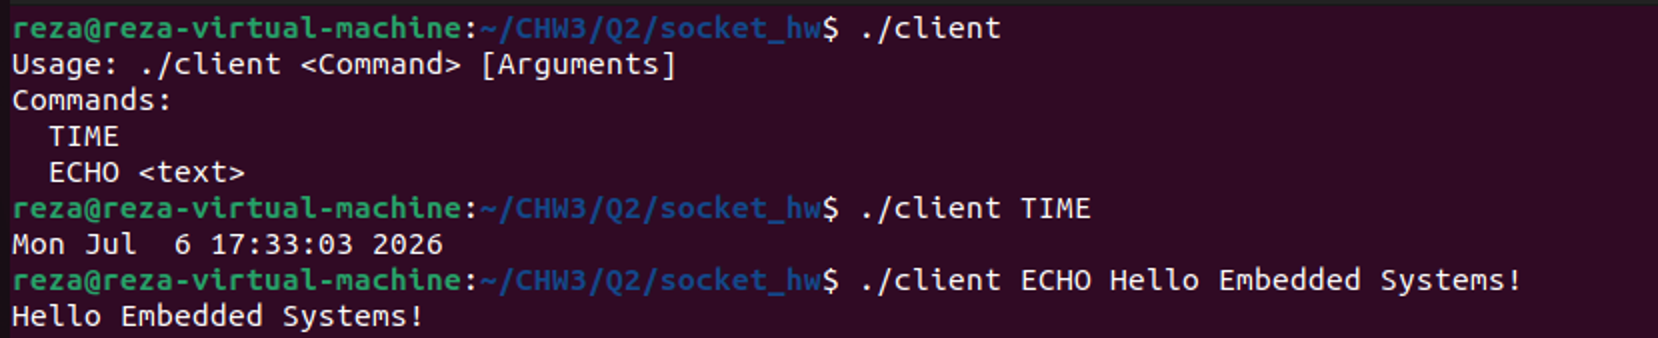
\includegraphics[width=\linewidth,height=.72\textheight,keepaspectratio]{assets/019_p019_01.png}\caption{Diagram or recorded result: procwatch code organization and build.}\label{fig:019_p019_010}\end{figure}
\begin{figure}[!htbp]\centering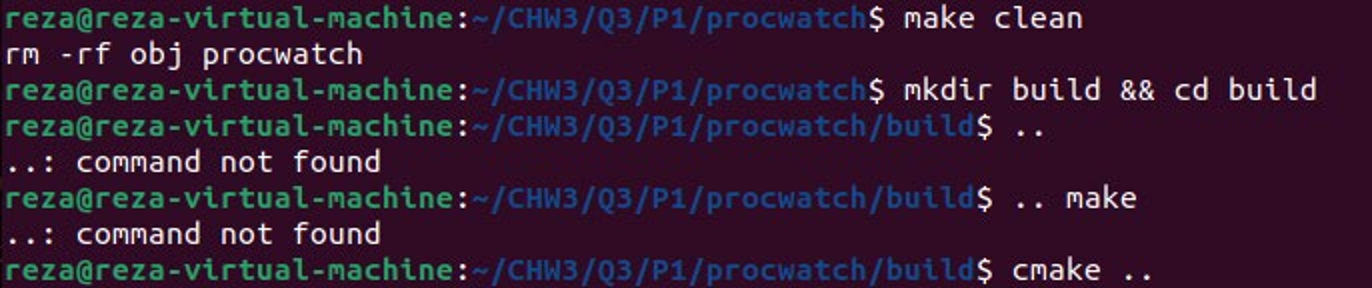
\includegraphics[width=\linewidth,height=.72\textheight,keepaspectratio]{assets/019_p020_01.png}\caption{Diagram or recorded result: procwatch code organization and build.}\label{fig:019_p020_010}\end{figure}
\begin{figure}[!htbp]\centering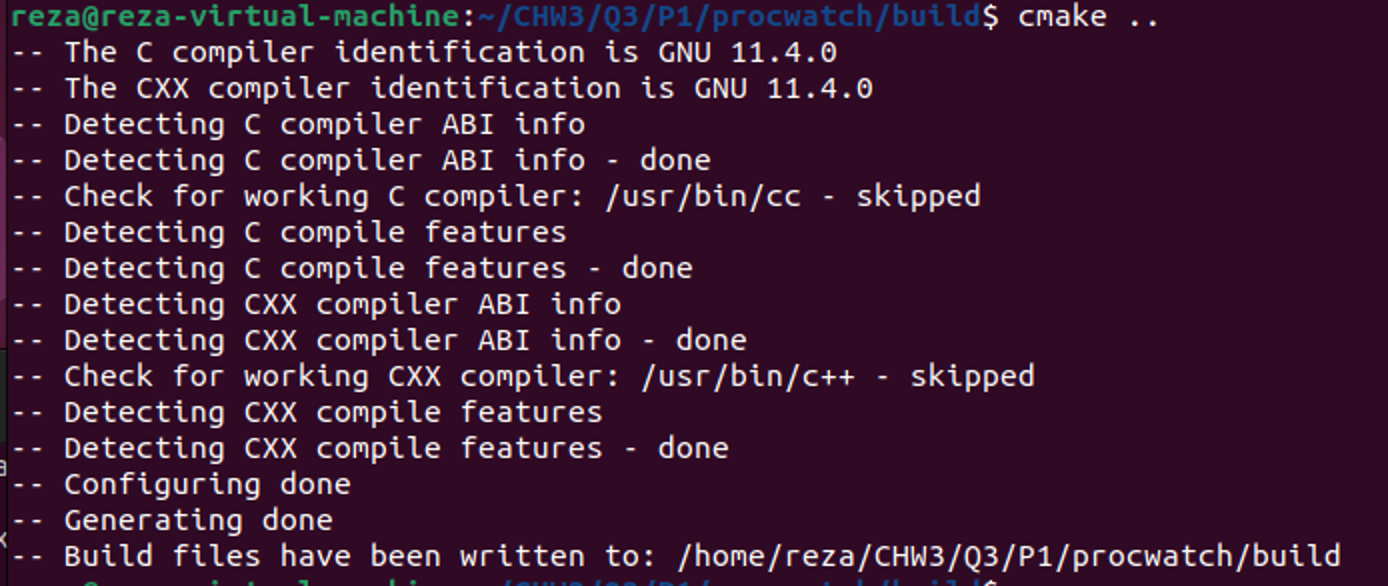
\includegraphics[width=\linewidth,height=.72\textheight,keepaspectratio]{assets/019_p020_02.png}\caption{Implementation and output: procwatch code organization and build.}\label{fig:019_p020_020}\end{figure}
\begin{figure}[!htbp]\centering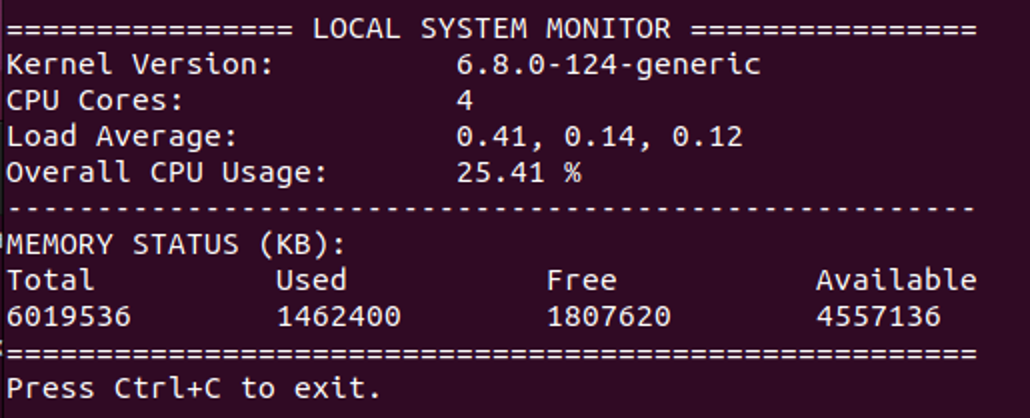
\includegraphics[width=\linewidth,height=.72\textheight,keepaspectratio]{assets/019_p020_03.png}\caption{Diagram or recorded result: procwatch code organization and build.}\label{fig:019_p020_030}\end{figure}
\begin{figure}[!htbp]\centering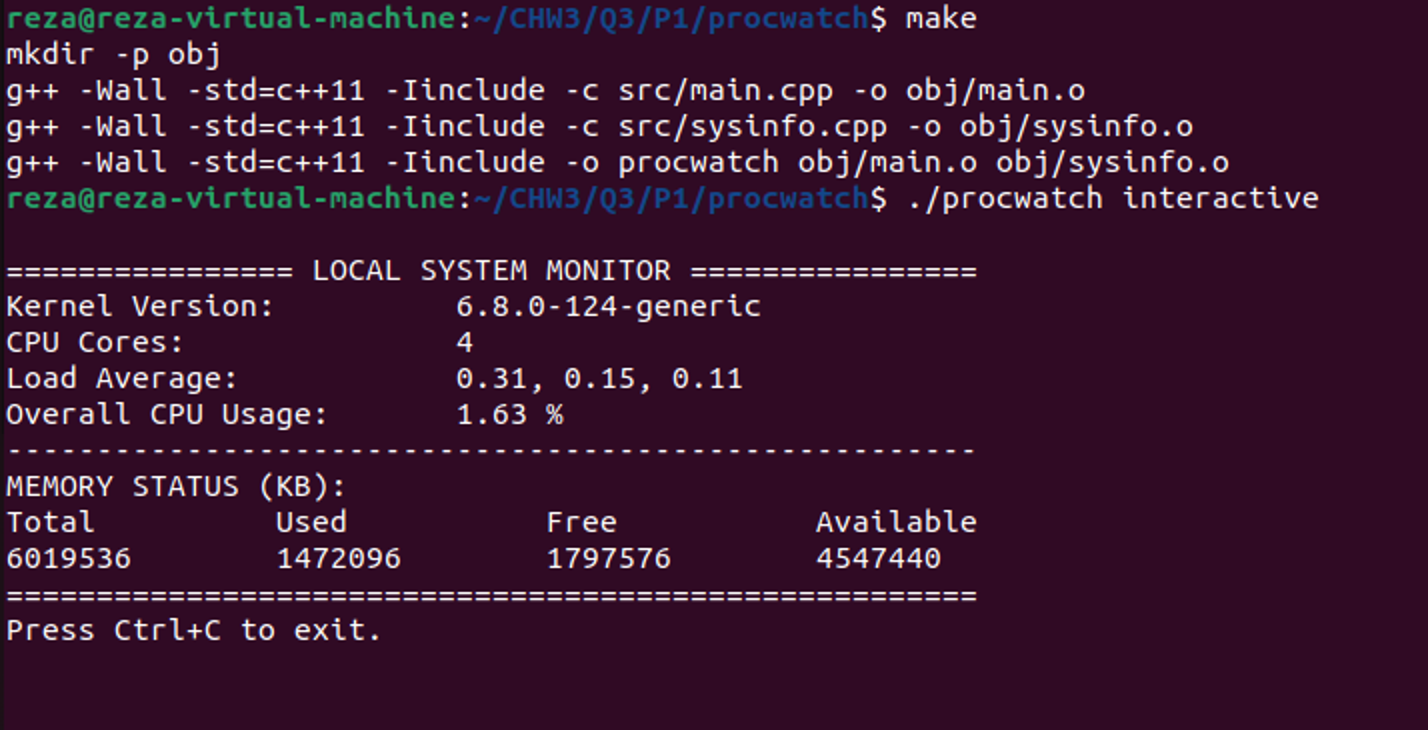
\includegraphics[width=\linewidth,height=.72\textheight,keepaspectratio]{assets/019_p020_04.png}\caption{Implementation and output: procwatch code organization and build.}\label{fig:019_p020_040}\end{figure}
\clearpage
\section{System telemetry and CPU calculation}

The interactive table reads kernel version from /\allowbreak{}proc/\allowbreak{}version, logical processor count from processor entries in /\allowbreak{}proc/\allowbreak{}cpuinfo, memory from /\allowbreak{}proc/\allowbreak{}meminfo, and one-, five-, and fifteen-minute load averages from /\allowbreak{}proc/\allowbreak{}loadavg. The recorded kernel is 6.8.0-124-generic. Used memory is estimated as MemTotal-MemAvailable;\allowbreak{} this is an available-capacity convention rather than a unique definition of all used memory. Load average is not the same as CPU percentage. The aggregate cpu line in /\allowbreak{}proc/\allowbreak{}stat contains cumulative user, nice, system, idle, iowait, irq, softirq, steal, and related counters. The code treats idle+\allowbreak{}iowait as idle and sums the selected busy counters separately. With consecutive samples, utilization is 100 times (DeltaTotal-DeltaIdle)/\allowbreak{}DeltaTotal. A single reading gives time accumulated since boot, not utilization over the last update. The interpretation of iowait and avoidance of double-counting guest fields should be explicit. At low activity the report records about 1.63 percent. With stress-ng --cpu 1 --timeout 30s on a four-logical-CPU system, htop shows one CPU near full use and procwatch reports 25.37 percent aggregate use. This is consistent with the expected approximately one-quarter aggregate busy time, allowing background activity and different sampling intervals. It is an informative cross-check rather than exact proof for every load pattern.

\begin{figure}[!htbp]\centering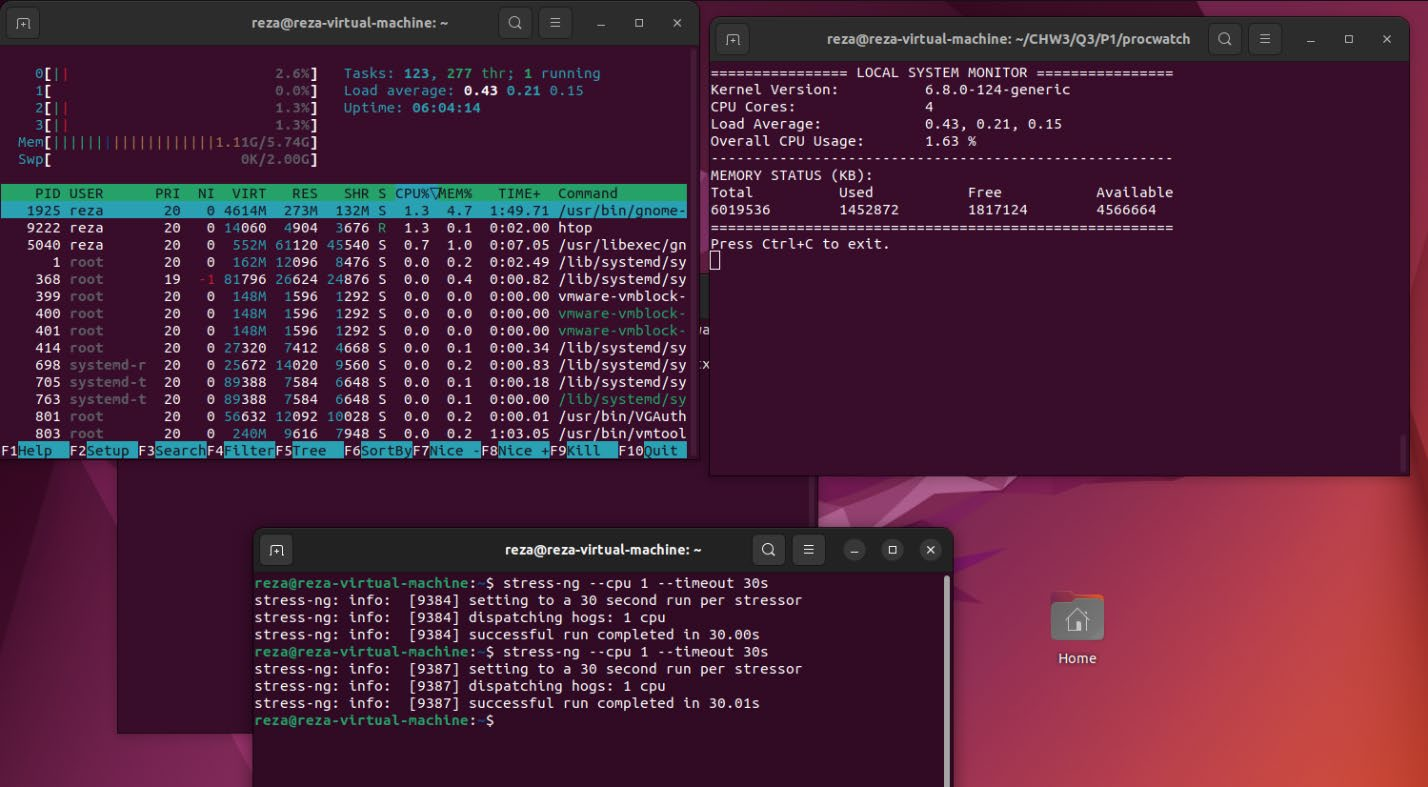
\includegraphics[width=\linewidth,height=.72\textheight,keepaspectratio]{assets/019_p023_01.png}\caption{Diagram or recorded result: System telemetry and CPU calculation.}\label{fig:019_p023_010}\end{figure}
\begin{figure}[!htbp]\centering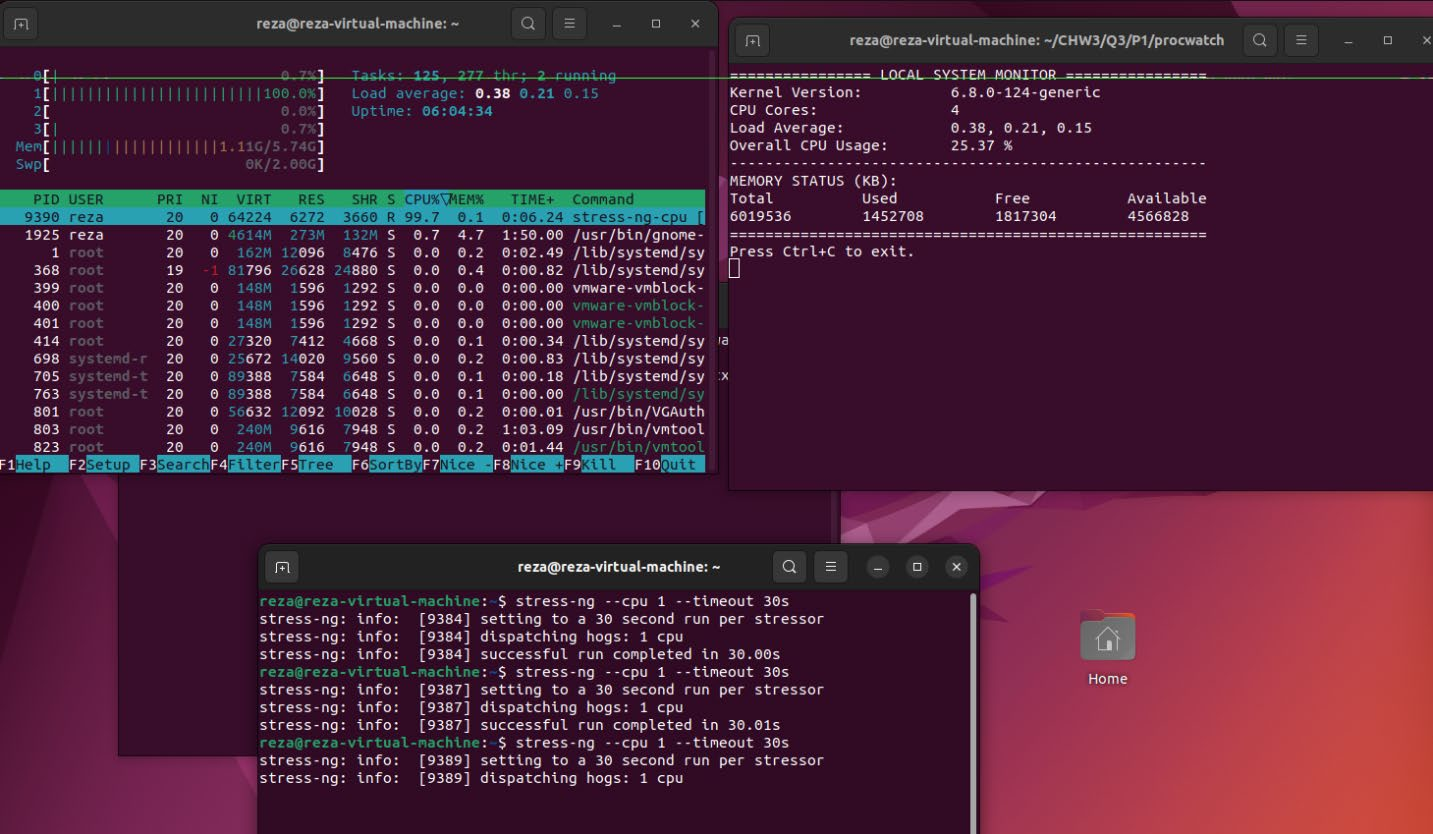
\includegraphics[width=\linewidth,height=.72\textheight,keepaspectratio]{assets/019_p024_01.png}\caption{Diagram or recorded result: System telemetry and CPU calculation.}\label{fig:019_p024_010}\end{figure}
\clearpage
\section{Per-process activity, names, and RSS}

Numeric /\allowbreak{}proc directory names identify candidate PIDs. The process name is parsed between the first opening and final closing parenthesis of /\allowbreak{}proc/\allowbreak{}[pid]/\allowbreak{}stat, which matters because names can contain spaces. Fields utime and stime give user/\allowbreak{}system CPU time;\allowbreak{} their consecutive differences provide interval activity. Previous values are retained in a map. Dividing a process's tick difference by aggregate system tick difference gives a percentage of total multicore capacity. For the familiar one-core-normalized top-style percentage, divide by elapsed wall time times the clock-tick rate, or account for logical CPU count consistently. RSS is read from the second field of /\allowbreak{}proc/\allowbreak{}[pid]/\allowbreak{}statm in pages and converted using sysconf(\_\allowbreak{}SC\_\allowbreak{}PAGESIZE), then into KiB. Four-KiB pages are common but not assumed. RSS measures resident pages and does not simply equal privately owned memory. Candidates are sorted by activity and the selected top N shown.

\begin{figure}[!htbp]\centering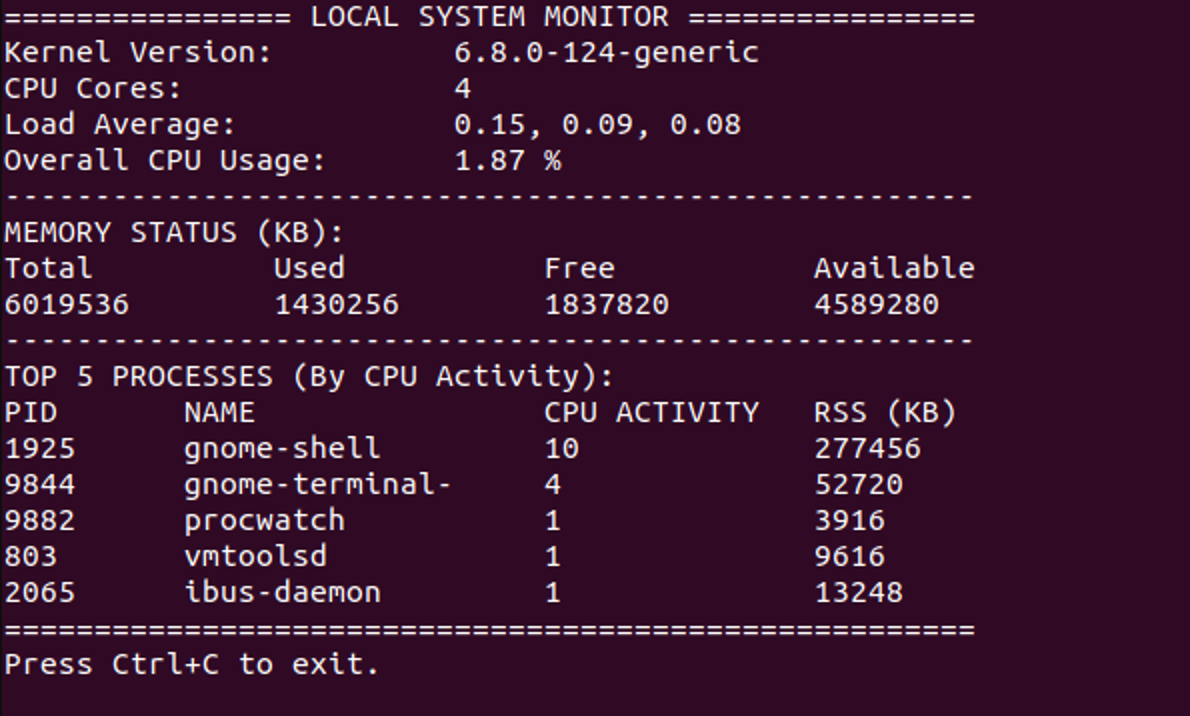
\includegraphics[width=\linewidth,height=.72\textheight,keepaspectratio]{assets/019_p025_01.png}\caption{Diagram or recorded result: Per-process activity, names, and RSS.}\label{fig:019_p025_010}\end{figure}
\begin{figure}[!htbp]\centering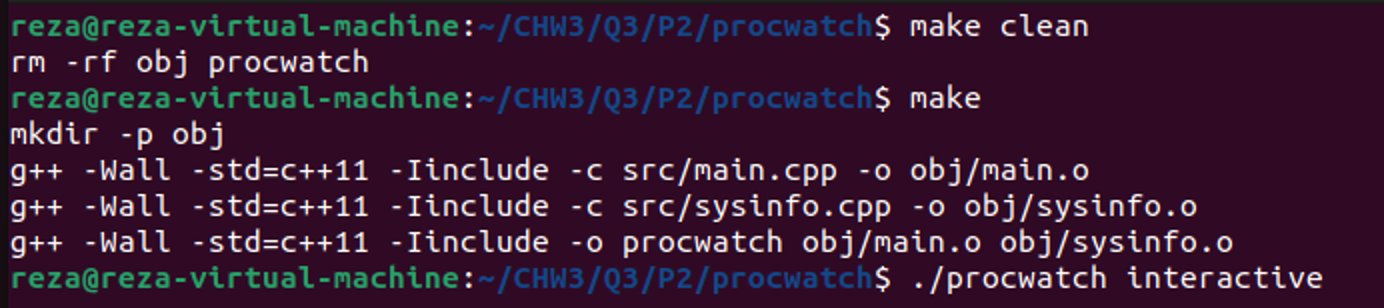
\includegraphics[width=\linewidth,height=.72\textheight,keepaspectratio]{assets/019_p025_02.png}\caption{Implementation and output: Per-process activity, names, and RSS.}\label{fig:019_p025_020}\end{figure}
\clearpage
\section{Dynamic /proc races}

A process can exit after enumeration but before its files are read. The program checks file-opening success and skips unavailable entries. This prevents the demonstrated missing-file path from crashing the monitor. Robust monitoring must also handle malformed/\allowbreak{}short reads, permission denial, PID reuse, changed counter baselines, and zero intervals. Skipping one common failure mode does not prove complete race freedom.

\section{Configuration, graceful termination, and restart tests}

The background configuration contains interval, n, and simulate\_\allowbreak{}error, and its path is passed on the command line. A SIGTERM handler sets a control flag so the loop exits, a shutdown message is recorded, and the process returns zero. The deliberate simulate\_\allowbreak{}error path exits with code one after several iterations. Signal handlers should restrict themselves to appropriate signal-safe operations;\allowbreak{} the ordinary loop should perform logging/\allowbreak{}cleanup.


procwatch.service selects background mode, uses Restart=\allowbreak{}on-failure, and sets RestartSec=\allowbreak{}5. In the ordinary test, a five-second interval and top-three output are recorded in the journal. In the fault test, the application logs CRITICAL:\allowbreak{} Simulated intentional error triggered! Exiting with code 1 and systemd restarts it approximately five seconds later. A successful SIGTERM termination and nonzero fault have different restart behavior. The evidence demonstrates these configured lifecycle paths, not resistance to every runtime failure.

\begin{figure}[!htbp]\centering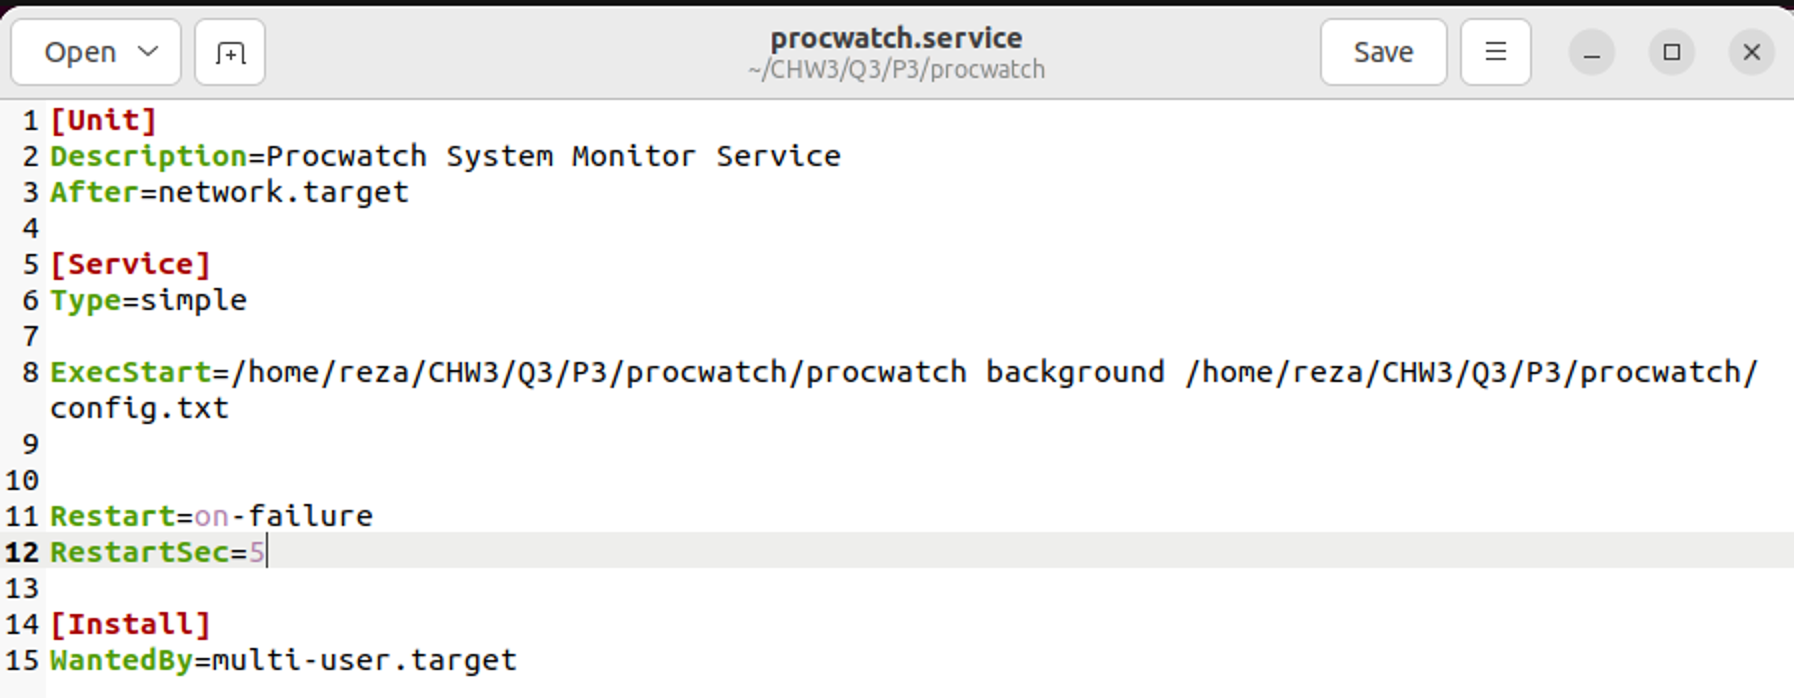
\includegraphics[width=\linewidth,height=.72\textheight,keepaspectratio]{assets/019_p028_01.png}\caption{Diagram or recorded result: Configuration, graceful termination, and restart tests.}\label{fig:019_p028_010}\end{figure}
\begin{figure}[!htbp]\centering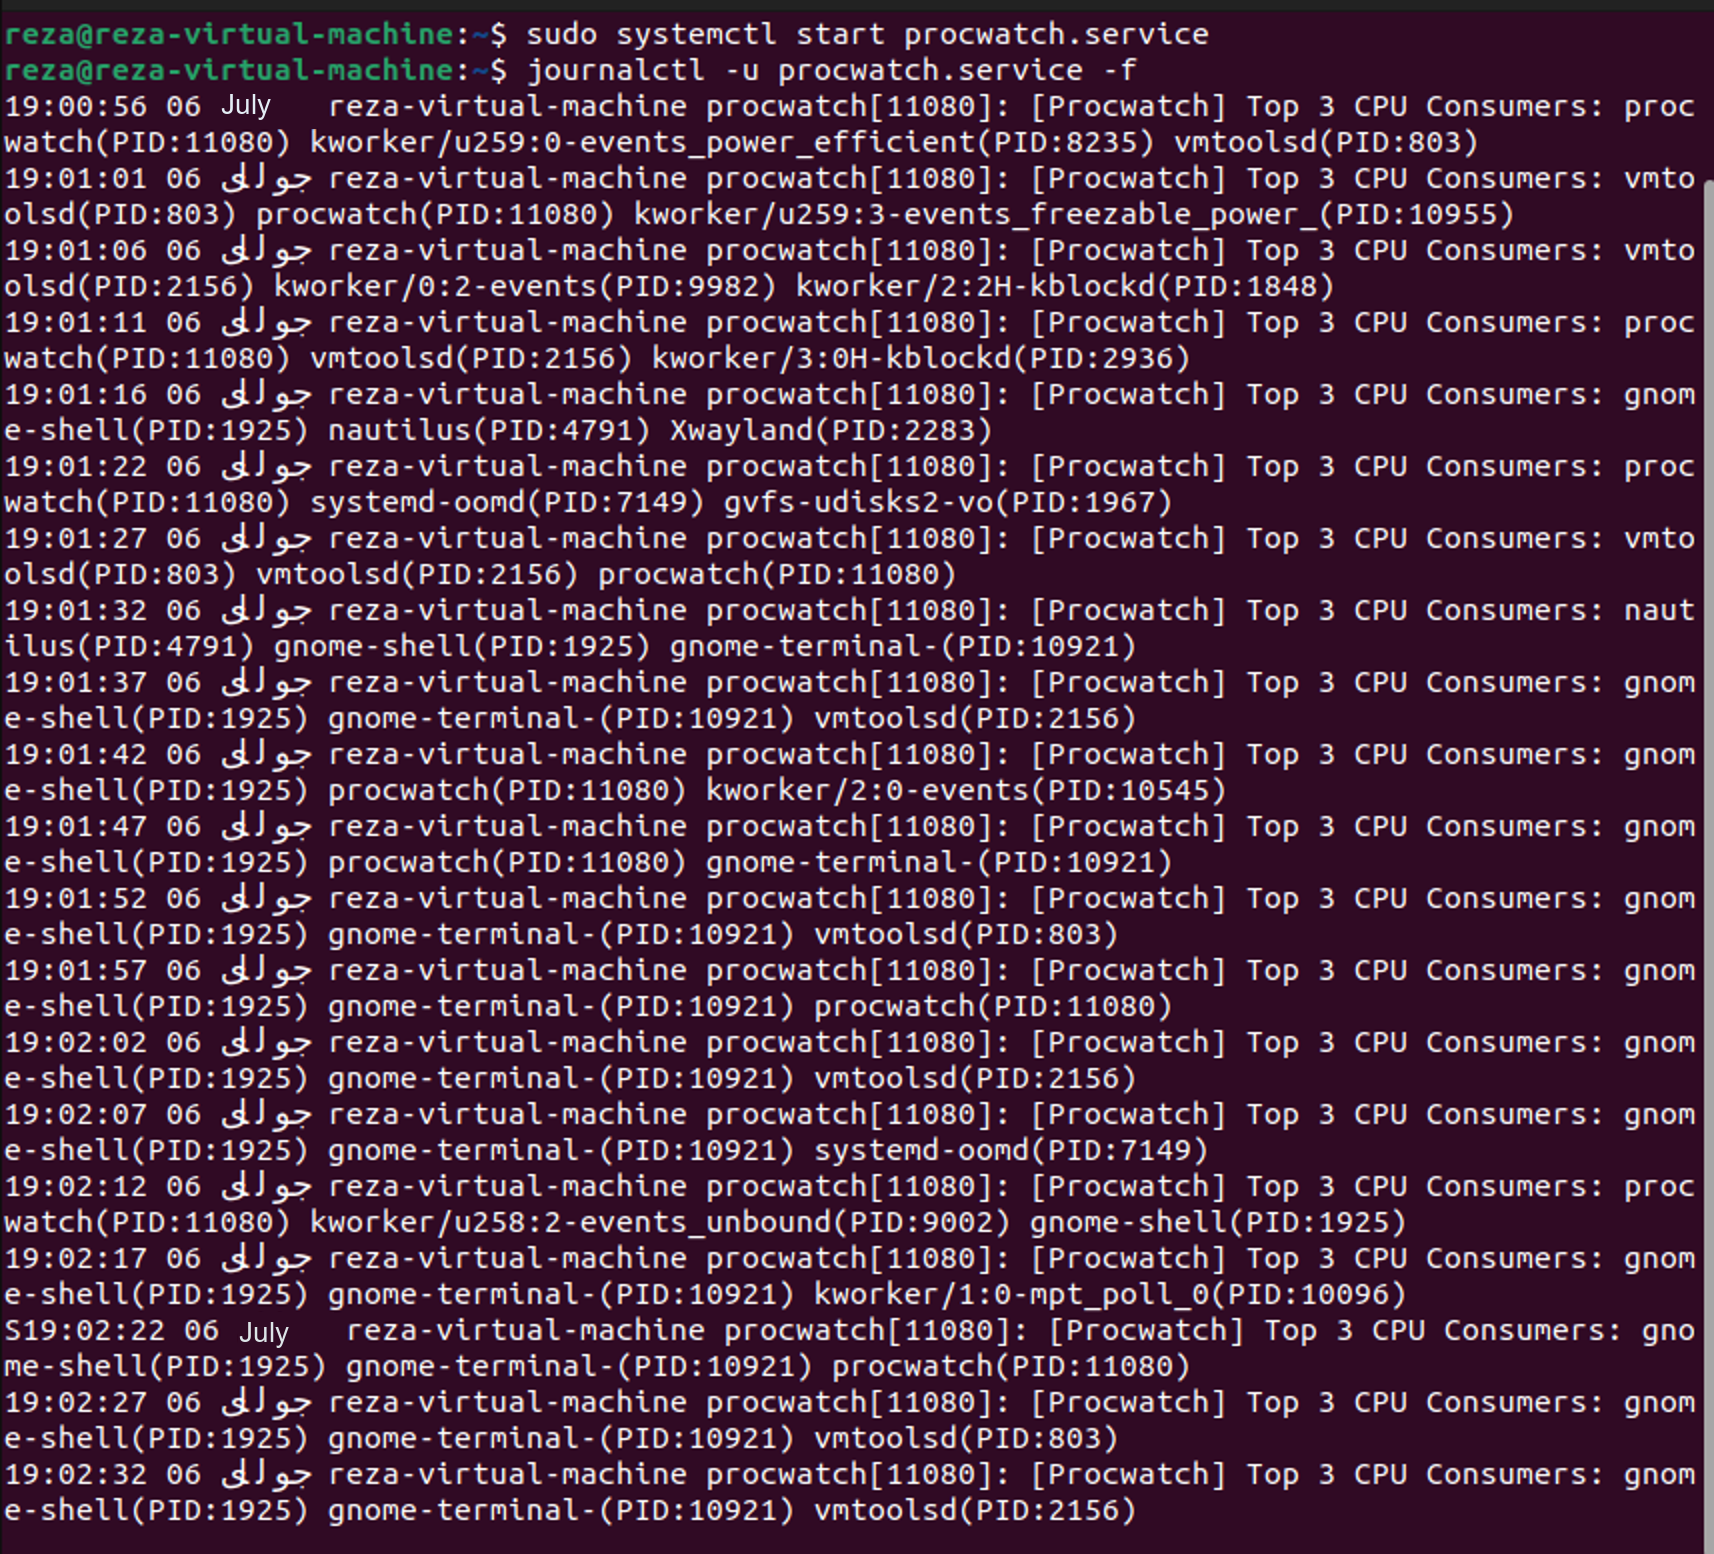
\includegraphics[width=\linewidth,height=.72\textheight,keepaspectratio]{assets/019_p029_01.png}\caption{Implementation and output: Configuration, graceful termination, and restart tests.}\label{fig:019_p029_010}\end{figure}
\begin{figure}[!htbp]\centering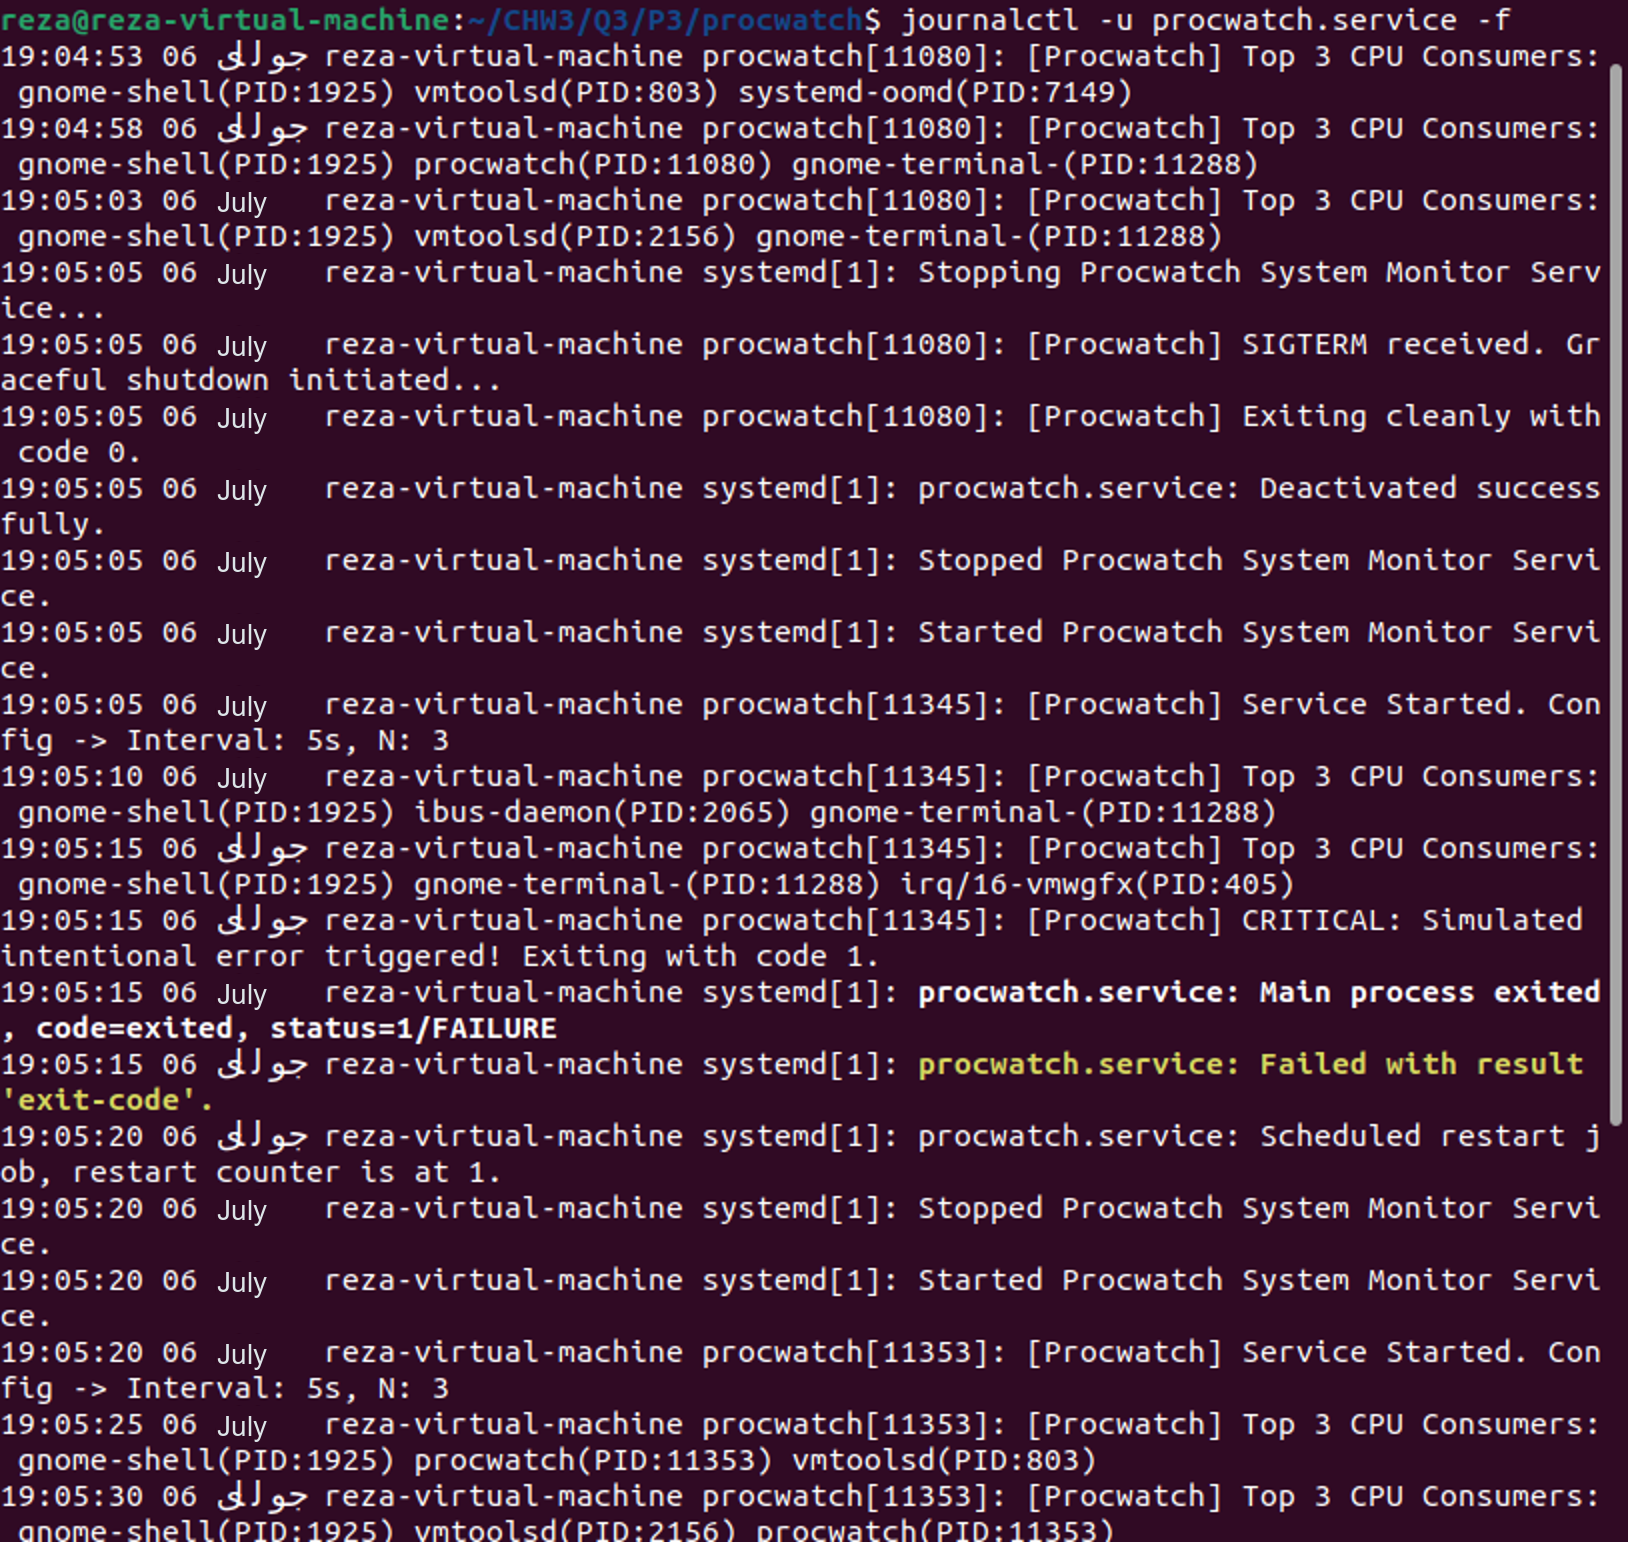
\includegraphics[width=\linewidth,height=.72\textheight,keepaspectratio]{assets/019_p030_01.png}\caption{Diagram or recorded result: Configuration, graceful termination, and restart tests.}\label{fig:019_p030_010}\end{figure}
\clearpage
\end{document}